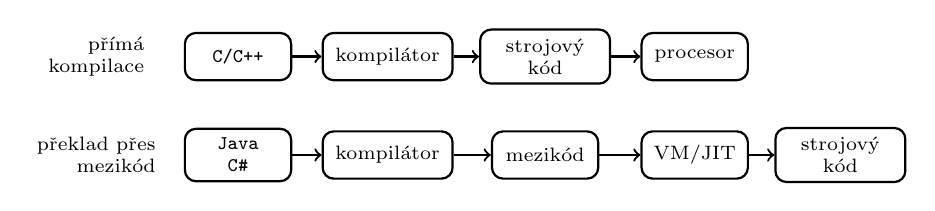
\begin{tikzpicture}[
    box/.style={
        draw,
        rounded corners,
        thick,
        align=center,
        font=\scriptsize,
        minimum width=1.35cm,
        minimum height=0.6cm
    },
    widebox/.style={
        draw,
        rounded corners,
        thick,
        align=center,
        font=\scriptsize,
        minimum width=1.65cm,
        minimum height=0.6cm
    },
    arrow/.style={->, thick}
]

    \visible<4->{
        \node[box] (c) at (0,0) {\texttt{C/C++}};
        \node[widebox] (comp1) at (1.9,0) {kompilátor};
        \node[widebox] (mc1) at (3.9,0) {strojový\\kód};
        \node[box] (cpu1) at (5.8,0) {procesor};

        \draw[arrow] (c) -- (comp1);
        \draw[arrow] (comp1) -- (mc1);
        \draw[arrow] (mc1) -- (cpu1);

        \node[font=\scriptsize, align=right] at (-1.8,0) {přímá\\kompilace};
    }

    \visible<7->{
        \node[box] (java) at (0,-1.25) {\texttt{Java}\\\texttt{C\#}};
        \node[widebox] (comp2) at (1.9,-1.25) {kompilátor};
        \node[box] (ir) at (3.9,-1.25) {mezikód};
        \node[box] (jit) at (5.8,-1.25) {VM/JIT};
        \node[widebox] (mc2) at (7.65,-1.25) {strojový\\kód};

        \draw[arrow] (java) -- (comp2);
        \draw[arrow] (comp2) -- (ir);
        \draw[arrow] (ir) -- (jit);
        \draw[arrow] (jit) -- (mc2);

        \node[font=\scriptsize, align=right] at (-1.8,-1.25) {překlad přes\\mezikód};
    }

\end{tikzpicture}
